

%\setcounter{chapter}{} 
% commands to check for inclusion 
% filter(), HoltWinters(), spectrum(), Box.test(), lag.plot(), monthplot(), tsdiag(),  
\chapter{LURN\ldots{} To Perform Times Series Analyses} 
\label{TimeSeries} 
 

 
This chapter focuses on some simple time series approaches for univariate time series. At this stage multivariate time series are not included, but could be in future depending on demand. In any case, the methods shown here are certainly not meant to be a comprehensive elucidation of all time series methods. Dealing with just the most commonly taught (and therefore the simplest) methods takes up enough space.  
 
You will need to refer to a standard time series analysis textbook for more complete guidance; many of these are now written with \R{} as the chosen software to support the material in the book. 
 
Given this proliferation of textbooks on the topic of time series analysis, it is no surprise that there are a number of add-on packages written to support them. In this chapter we do not extend beyond the functionality offered by the base distribution of \R{}. 
 
\section{Time series objects in \R{}} 
 
The basic univariate time series, with no missing data is stored in \R{} as a time series object. This is marginally different to a vector in that it has a time stamp or index associated with each observation in the series. 
 
We will use several time series data sets that are available within the default installation of \R{}.  
\begin{knitrout}
\definecolor{shadecolor}{rgb}{0.969, 0.969, 0.969}\color{fgcolor}\begin{kframe}
\begin{alltt}
\hlstd{> }\hlkwd{str}\hlstd{(LakeHuron)}
\end{alltt}
\begin{verbatim}
 Time-Series [1:98] from 1875 to 1972: 580 582 581 581 580 ...
\end{verbatim}
\begin{alltt}
\hlstd{> }\hlkwd{str}\hlstd{(lynx)}
\end{alltt}
\begin{verbatim}
 Time-Series [1:114] from 1821 to 1934: 269 321 585 871 1475 ...
\end{verbatim}
\begin{alltt}
\hlstd{> }\hlkwd{str}\hlstd{(Nile)}
\end{alltt}
\begin{verbatim}
 Time-Series [1:100] from 1871 to 1970: 1120 1160 963 1210 1160 1160 813 1230 1370 1140 ...
\end{verbatim}
\end{kframe}
\end{knitrout}
The first is for the level of Lake Huron; the second is the number of lynx that were trapped in Canada; and the third is the flow of the River Nile. More detailed information for all of these series is available using the relevant help function for the series. 
 
You can use the Rcmd{as.ts} command to convert a vector of observations to a time series object. For example, the Robject{airquality} data is recorded in time order. We might want to treat the observed temperatures as a time series by converting it using: 
\begin{knitrout}
\definecolor{shadecolor}{rgb}{0.969, 0.969, 0.969}\color{fgcolor}\begin{kframe}
\begin{alltt}
\hlstd{> }\hlstd{Temp.ts} \hlkwb{=} \hlkwd{as.ts}\hlstd{(airquality}\hlopt{$}\hlstd{Temp)}
\end{alltt}
\end{kframe}
\end{knitrout}
 
\section{Time series plots} 
 
We have seen the flexibility of the \Rcmd{plot} command in previous chapters, and now we see another use. Applying the \Rcmd{plot} command to a time series object generates a time series plot, as seen in Exhibit~\ref{NileTSPlot}. 
\begin{exhibit} 
\begin{center} 
\caption{Time series plot for the annual flow of the River Nile.} 
\label{NileTSPlot} 
\begin{knitrout}
\definecolor{shadecolor}{rgb}{0.969, 0.969, 0.969}\color{fgcolor}\begin{kframe}
\begin{alltt}
\hlstd{> }\hlkwd{plot}\hlstd{(Nile,} \hlkwc{xlab}\hlstd{=}\hlstr{"Year"}\hlstd{,} \hlkwc{ylab}\hlstd{=}\hlstr{"Flow"}\hlstd{)}
\end{alltt}
\end{kframe}
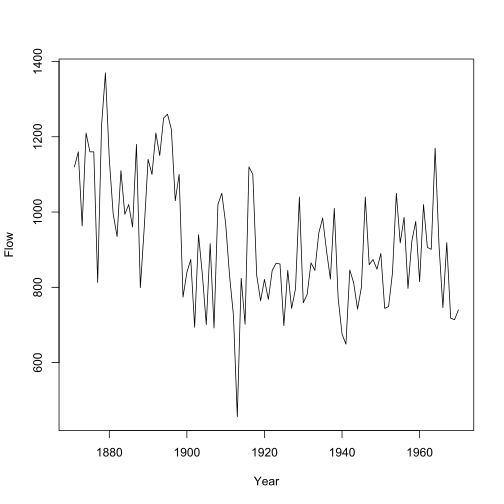
\includegraphics[width=0.7\textwidth]{figures/TimeSeriesNilePlot-1} 

\end{knitrout}
\SVGLink{TimeSeriesNilePlot-1} 
\end{center} 
\end{exhibit} 
%%%check resulting graph and fix 
 
Having the class assigned to our data means the plot was enhanced slightly. Check this by comparing the results for the two plots in Exhibit~\ref{TSPlotsCompared}. 
\begin{exhibit} 
\begin{center} 
\caption{Comparison of use of \Rcmd{plot} on a vector and a time series object.} 
\label{TSPlotsCompared} 
\begin{knitrout}
\definecolor{shadecolor}{rgb}{0.969, 0.969, 0.969}\color{fgcolor}\begin{kframe}
\begin{alltt}
\hlstd{> }\hlkwd{plot}\hlstd{(airquality}\hlopt{$}\hlstd{Temp,} \hlkwc{ylab}\hlstd{=}\hlstr{"Temperature"}\hlstd{)}
\end{alltt}
\end{kframe}
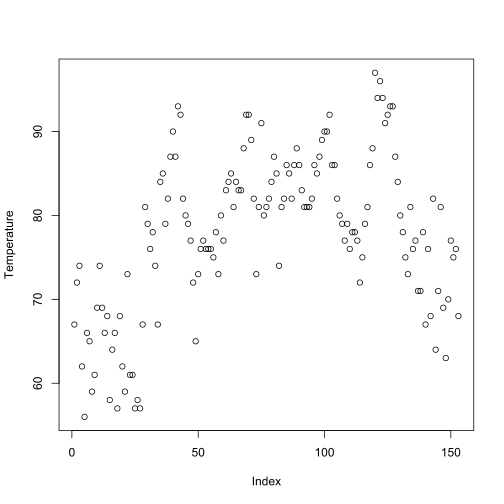
\includegraphics[width=0.7\textwidth]{figures/TimeSeriesTSPlotsCompared-1} 
\begin{kframe}\begin{alltt}
\hlstd{> }\hlkwd{plot}\hlstd{(Temp.ts,} \hlkwc{ylab}\hlstd{=}\hlstr{"Temperature"}\hlstd{)}
\end{alltt}
\end{kframe}
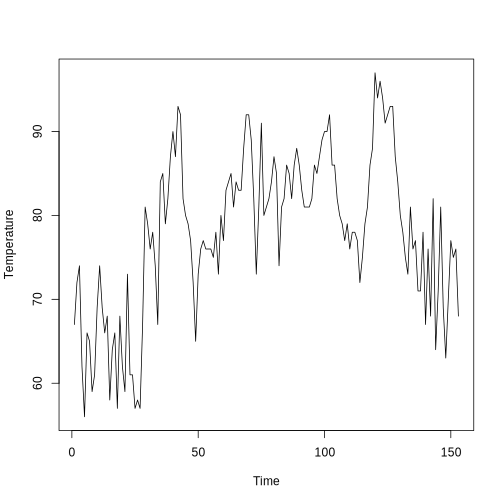
\includegraphics[width=0.7\textwidth]{figures/TimeSeriesTSPlotsCompared-2} 

\end{knitrout}
\SVGLink{TSPlotsCompared-1} 
\SVGLink{TSPlotsCompared-2} 
\end{center} 
\end{exhibit} 
 
\section{Smoothing of a time series using moving averages} 
 
One simple method for smoothing out a time series in order to expose its behaviour is to smooth out the observed data using  the \Rcmd{filter} command to create a moving average. 
A moving average is often centred, (using the argument \Rarg{sides=2}) but if the series is expected to have no trend, then a backwards only (\Rarg{sides=1})  focus can be taken. We must determine the width of the moving average, usually using odd-numbered widths. 
 
Exhibit~\ref{FilterExample} shows how different amounts of data can be averaged to change the amount of smoothing. 
\begin{exhibit} 
\begin{center} 
\caption{Comparison of different amounts of smoothing a time series.} 
\label{FilterExample} 
\begin{knitrout}
\definecolor{shadecolor}{rgb}{0.969, 0.969, 0.969}\color{fgcolor}\begin{kframe}
\begin{alltt}
\hlstd{> }\hlkwd{plot}\hlstd{(Nile)}
\end{alltt}
\end{kframe}
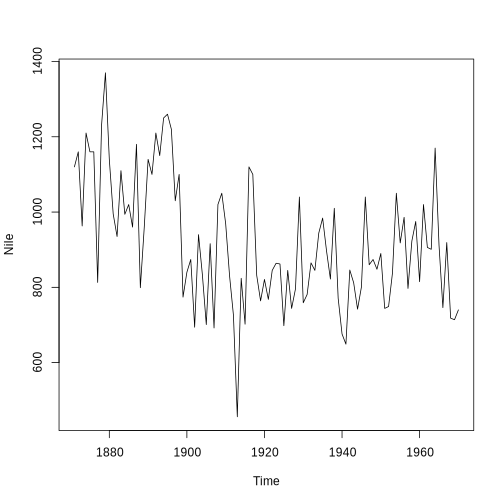
\includegraphics[width=0.7\textwidth]{figures/TimeSeriesFilterExample-1} 
\begin{kframe}\begin{alltt}
\hlstd{> }\hlkwa{for}\hlstd{(i} \hlkwa{in} \hlnum{1}\hlopt{:}\hlnum{4}\hlstd{)\{}
\hlstd{   }\hlstd{w}\hlkwb{=}\hlnum{4}\hlopt{*}\hlstd{i}\hlopt{-}\hlnum{1} \hlcom{# choose the window (3, 7,11,15) }
\hlstd{   }\hlkwd{lines}\hlstd{( (}\hlkwd{start}\hlstd{(Nile)[}\hlnum{1}\hlstd{])}\hlopt{:}\hlkwd{end}\hlstd{(Nile)[}\hlnum{1}\hlstd{],} \hlkwd{filter}\hlstd{(Nile,} \hlkwd{rep}\hlstd{(}\hlnum{1}\hlopt{/}\hlstd{w, w),} \hlkwc{sides}\hlstd{=}\hlnum{1}\hlstd{),} \hlkwc{col}\hlstd{=i}\hlopt{+}\hlnum{2}\hlstd{)}
\hlstd{   }\hlstd{\}}
\end{alltt}


{\ttfamily\noindent\bfseries\color{errorcolor}{Error in UseMethod("{}filter\_"{}): no applicable method for 'filter\_' applied to an object of class "{}ts"{}}}\end{kframe}
\end{knitrout}
\SVGLink{FilterExample-1} 
\end{center} 
\end{exhibit} 
 
\section{Checking for stationarity}\label{Stationarity}  
 
\stress{Stationarity} is important for modelling time series. Some descriptive methods also need it. 
The simplest form of \nostressind{stationarity} is when the mean of the series and the variance of the series both remain roughly constant over time, or as explained by Hyndman and Athana-sopou-los (2013), "[a] stationary time series is one whose properties do not depend on the time at which the series is observed". (their book is called Forecasting: Principles and Practice.) 
  
A \stressind{white noise} series of normally distributed data with mean zero and constant variance $\sigma^2$ is the strongest form of stationarity we seek in our modelling. It is the desired outcome for the residuals from any model we fit to time series data. 
 
 
The \Rcmd{Box.test} function tests for non-stationarity. 
\begin{knitrout}
\definecolor{shadecolor}{rgb}{0.969, 0.969, 0.969}\color{fgcolor}\begin{kframe}
\begin{alltt}
\hlstd{> }\hlkwd{Box.test}\hlstd{(Nile,} \hlkwc{lag}\hlstd{=}\hlnum{20}\hlstd{)}
\end{alltt}
\begin{verbatim}

	Box-Pierce test

data:  Nile
X-squared = 120, df = 20, p-value = 1e-15
\end{verbatim}
\end{kframe}
\end{knitrout}
while several other tests exist in add-on packages which can be accessed by loading the  Rpkg{tseries} and \Rpkgforecast} packages. 
\begin{knitrout}
\definecolor{shadecolor}{rgb}{0.969, 0.969, 0.969}\color{fgcolor}\begin{kframe}
\begin{alltt}
\hlstd{> }\hlkwd{library}\hlstd{(tseries)}
\hlstd{> }\hlkwd{library}\hlstd{(forecast)}
\end{alltt}


{\ttfamily\noindent\itshape\color{messagecolor}{Loading required package: zoo}}

{\ttfamily\noindent\itshape\color{messagecolor}{\\Attaching package: 'zoo'}}

{\ttfamily\noindent\itshape\color{messagecolor}{The following objects are masked from 'package:base':

\ \ \ \ as.Date, as.Date.numeric}}

{\ttfamily\noindent\itshape\color{messagecolor}{Loading required package: timeDate}}

{\ttfamily\noindent\itshape\color{messagecolor}{This is forecast 7.1 }}\begin{alltt}
\hlstd{> }\hlkwd{adf.test}\hlstd{(Nile)}
\end{alltt}
\begin{verbatim}

	Augmented Dickey-Fuller Test

data:  Nile
Dickey-Fuller = -3.4, Lag order = 4, p-value = 0.06
alternative hypothesis: stationary
\end{verbatim}
\begin{alltt}
\hlstd{> }\hlkwd{pp.test}\hlstd{(Nile)}
\end{alltt}


{\ttfamily\noindent\color{warningcolor}{Warning in pp.test(Nile): p-value smaller than printed p-value}}\begin{verbatim}

	Phillips-Perron Unit Root Test

data:  Nile
Dickey-Fuller Z(alpha) = -65, Truncation lag
parameter = 3, p-value = 0.01
alternative hypothesis: stationary
\end{verbatim}
\begin{alltt}
\hlstd{> }\hlkwd{kpss.test}\hlstd{(Nile)}
\end{alltt}


{\ttfamily\noindent\color{warningcolor}{Warning in kpss.test(Nile): p-value smaller than printed p-value}}\begin{verbatim}

	KPSS Test for Level Stationarity

data:  Nile
KPSS Level = 1.3, Truncation lag parameter = 2,
p-value = 0.01
\end{verbatim}
\end{kframe}
\end{knitrout}
Each test is looking at a different facet of what might indicate how a series might not be stationary. Check out the null hypothesis and alternative for each test on its help page. 
 
 
%% diff() 
 
\section{Autocorrelation and partial autocorrelation} 
 
% check out the Box.test() command. 
 
The autocorrelation and partial autocorrelation function values can be obtained using the \Rcmd{acf} and \Rcmd{pacf} commands. Plotting these is a common way to determine if any of the values found are of interest in understanding the process being modelled so this is the default action performed by these commands. See Exhibit~\ref{NileACF} for the plot generated by the \Rcmd{acf} command. The \Rcmd{pacf} command functions in the same way so is not demonstrated. 
\begin{exhibit} 
\begin{center} 
\caption{Autocorrelation function for the annual flow of the River Nile.} 
\label{NileACF} 
\begin{knitrout}
\definecolor{shadecolor}{rgb}{0.969, 0.969, 0.969}\color{fgcolor}\begin{kframe}
\begin{alltt}
\hlstd{> }\hlkwd{acf}\hlstd{(Nile)}
\end{alltt}
\end{kframe}
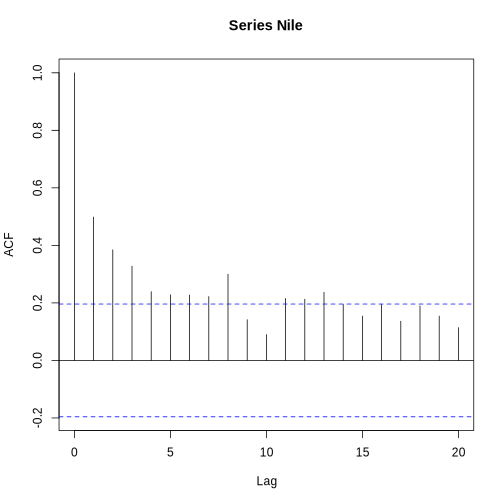
\includegraphics[width=0.7\textwidth]{figures/TimeSeriesNileACF-1} 

\end{knitrout}
\SVGLink{TimeSeriesNileACF-1} 
\end{center} 
\end{exhibit} 
 
To obtain the values of the autocorrelation function (or partial autocorrelation function) in text form, we add an argument to stop the results being plotted. 
\begin{knitrout}
\definecolor{shadecolor}{rgb}{0.969, 0.969, 0.969}\color{fgcolor}\begin{kframe}
\begin{alltt}
\hlstd{> }\hlkwd{acf}\hlstd{(Nile,} \hlkwc{plot}\hlstd{=}\hlnum{FALSE}\hlstd{)}
\end{alltt}
\begin{verbatim}

Autocorrelations of series 'Nile', by lag

    0     1     2     3     4     5     6     7     8     9 
1.000 0.498 0.385 0.328 0.239 0.228 0.227 0.222 0.300 0.142 
   10    11    12    13    14    15    16    17    18    19 
0.090 0.215 0.213 0.237 0.195 0.154 0.195 0.136 0.190 0.154 
   20 
0.114 
\end{verbatim}
\begin{alltt}
\hlstd{> }\hlkwd{pacf}\hlstd{(Nile,} \hlkwc{plot}\hlstd{=}\hlnum{FALSE}\hlstd{)}
\end{alltt}
\begin{verbatim}

Partial autocorrelations of series 'Nile', by lag

     1      2      3      4      5      6      7      8 
 0.498  0.181  0.111  0.006  0.065  0.071  0.060  0.163 
     9     10     11     12     13     14     15     16 
-0.148 -0.065  0.190  0.087  0.065 -0.053 -0.030  0.073 
    17     18     19     20 
 0.017  0.115 -0.124 -0.059 
\end{verbatim}
\end{kframe}
\end{knitrout}
 
\section{Decomposition into seasonal and trend components} 
 
The basic idea of the decompositions presented in this section is to explain the observed time series values $y_t$ in terms of a trend $T_t$, a seasonal component $S_t$ and residual error. 
 
Obviously we need a series that has a seasonal component such as the Australian resident numbers measured quarterly from  1971 to 1994. 
\begin{knitrout}
\definecolor{shadecolor}{rgb}{0.969, 0.969, 0.969}\color{fgcolor}\begin{kframe}
\begin{alltt}
\hlstd{> }\hlkwd{str}\hlstd{(austres)}
\end{alltt}
\begin{verbatim}
 Time-Series [1:89] from 1971 to 1993: 13067 13130 13198 13254 13304 ...
\end{verbatim}
\end{kframe}
\end{knitrout}
 
 
The \Rcmd{decompose} function can create two forms of the decomposition, one of which is additive and the other is multiplicative. 
\begin{knitrout}
\definecolor{shadecolor}{rgb}{0.969, 0.969, 0.969}\color{fgcolor}\begin{kframe}
\begin{alltt}
\hlstd{> }\hlstd{AustRes.dec1} \hlkwb{=} \hlkwd{decompose}\hlstd{(austres)}
\hlstd{> }\hlstd{Aust.dec2} \hlkwb{=}\hlkwd{decompose}\hlstd{(austres,} \hlkwc{type}\hlstd{=}\hlstr{"mul"}\hlstd{)}
\end{alltt}
\end{kframe}
\end{knitrout}
The Rcmd{stl} command uses loess smoothing to estimate the trend component before finding the seasonal components and the resulting error terms, and is a slightly more advanced process than that offered by \Rcmd{decompose(}. N.B. there is an \Rcmd{stl} command in the \Rpkg{stats} package and another in the \Rpkg{forecast} package. We use the simpler one here but need to force \R{} to do so just in case the \Rpkg{forecast} package version has precedence. 
 
\begin{knitrout}
\definecolor{shadecolor}{rgb}{0.969, 0.969, 0.969}\color{fgcolor}\begin{kframe}
\begin{alltt}
\hlstd{> }\hlstd{AustRes.dec3} \hlkwb{=} \hlstd{stats}\hlopt{::}\hlkwd{stl}\hlstd{(austres,} \hlkwc{s.window}\hlstd{=}\hlstr{"periodic"}\hlstd{)}
\hlstd{> }\hlstd{AustRes.dec3}
\end{alltt}
\begin{verbatim}
 Call:
 stats::stl(x = austres, s.window = "periodic")

Components
        seasonal trend remainder
1971 Q2  -0.9674 13075   -6.3062
1971 Q3  -8.1113 13133    5.3950
1971 Q4   0.2031 13192    6.5849
1972 Q1   8.8756 13249   -4.1298
1972 Q2  -0.9674 13304    0.7167
1972 Q3  -8.1113 13357    5.4690
1972 Q4   0.2031 13407    2.3083
1973 Q1   8.8756 13456   -5.7763
1973 Q2  -0.9674 13507   -1.2525
1973 Q3  -8.1113 13559    1.5244
1973 Q4   0.2031 13612    1.6742
1974 Q1   8.8756 13667   -6.1772
1974 Q2  -0.9674 13722    1.7391
1974 Q3  -8.1113 13774    5.9067
1974 Q4   0.2031 13820   12.2123
1975 Q1   8.8756 13859   -5.4636
1975 Q2  -0.9674 13895   -1.4363
1975 Q3  -8.1113 13931    3.8638
1975 Q4   0.2031 13966    2.6435
1976 Q1   8.8756 14000   -4.5882
1976 Q2  -0.9674 14036   -1.5082
1976 Q3  -8.1113 14072    1.6595
1976 Q4   0.2031 14111   -1.0116
1977 Q1   8.8756 14151   -4.5138
1977 Q2  -0.9674 14194   -0.5377
1977 Q3  -8.1113 14237    2.4705
1977 Q4   0.2031 14280    1.2646
1978 Q1   8.8756 14321    0.1618
1978 Q2  -0.9674 14361   -0.5714
1978 Q3  -8.1113 14398    6.6065
1978 Q4   0.2031 14436   -4.9187
1979 Q1   8.8756 14474   -4.9753
1979 Q2  -0.9674 14516    0.2490
1979 Q3  -8.1113 14559    3.7081
1979 Q4   0.2031 14602    0.1959
1980 Q1   8.8756 14648  -10.3244
1980 Q2  -0.9674 14698   -1.5489
1980 Q3  -8.1113 14753    2.1397
1980 Q4   0.2031 14809   -2.1222
1981 Q1   8.8756 14868   -2.1550
1981 Q2  -0.9674 14929   -4.7949
1981 Q3  -8.1113 14991    5.4915
1981 Q4   0.2031 15055   -0.6364
1982 Q1   8.8756 15118   -5.2979
1982 Q2  -0.9674 15180    5.3648
1982 Q3  -8.1113 15238    9.8432
1982 Q4   0.2031 15291   -2.1066
1983 Q1   8.8756 15341   -4.1717
1983 Q2  -0.9674 15392    2.8485
1983 Q3  -8.1113 15439    7.6489
1983 Q4   0.2031 15485   -1.6301
1984 Q1   8.8756 15531   -8.5709
1984 Q2  -0.9674 15580    0.4185
1984 Q3  -8.1113 15630    6.3188
1984 Q4   0.2031 15681   -4.1708
1985 Q1   8.8756 15733   -5.6262
1985 Q2  -0.9674 15788    0.8474
1985 Q3  -8.1113 15845    3.0458
1985 Q4   0.2031 15901   -0.6827
1986 Q1   8.8756 15959   -6.4548
1986 Q2  -0.9674 16019    0.1646
1986 Q3  -8.1113 16080    5.3946
1986 Q4   0.2031 16140   -0.9897
1987 Q1   8.8756 16201   -7.0776
1987 Q2  -0.9674 16266   -1.3068
1987 Q3  -8.1113 16333    3.1703
1987 Q4   0.2031 16401   -2.6662
1988 Q1   8.8756 16472   -2.4364
1988 Q2  -0.9674 16546   -7.0499
1988 Q3  -8.1113 16622    8.1829
1988 Q4   0.2031 16696    0.8982
1989 Q1   8.8756 16766    2.2061
1989 Q2  -0.9674 16833    1.5003
1989 Q3  -8.1113 16896    3.6136
1989 Q4   0.2031 16958   -1.7351
1990 Q1   8.8756 17017   -0.0670
1990 Q2  -0.9674 17071   15.0287
1990 Q3  -8.1113 17123   -8.3421
1990 Q4   0.2031 17175   -5.9274
1991 Q1   8.8756 17232   -1.9143
1991 Q2  -0.9674 17294   -1.4950
1991 Q3  -8.1113 17352   10.0977
1991 Q4   0.2031 17402   12.1373
1992 Q1   8.8756 17446   -7.2696
1992 Q2  -0.9674 17486   -2.9214
1992 Q3  -8.1113 17529    5.3008
1992 Q4   0.2031 17573   -4.7695
1993 Q1   8.8756 17618    0.7089
1993 Q2  -0.9674 17662    0.7065
\end{verbatim}
\begin{alltt}
\hlstd{> }\hlkwd{plot}\hlstd{(AustRes.dec3)}
\end{alltt}
\end{kframe}
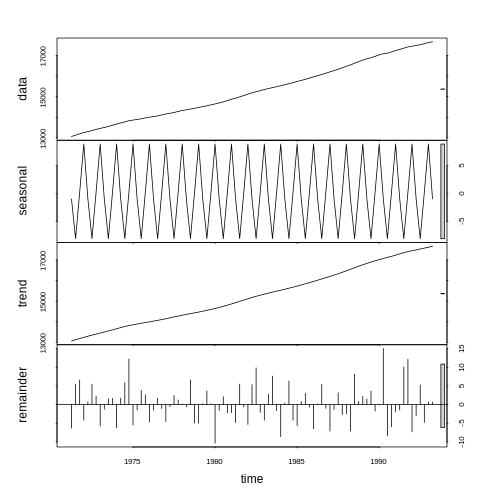
\includegraphics[width=0.7\textwidth]{figures/TimeSeriesSTLAustRes-1} 

\end{knitrout}
 
\section{Exponential smoothing} 
 
Exponential smoothing is a method for making predictions of the next observation in a time series. The next observation is a weighted average of all observations to date, with the most recent given the greatest weight and the oldest ones having the least impact. This simple version is useful for situations with no seasonal component or systematic trend component. 
 
Note that this is often expressed as $$\hat{y}_{t+1} = \lambda \hat{y}_{t} + (1-\lambda)y_{t}$$ 
Substituting for $\hat{y}_t$ in terms of terms at time ***t-1*** shows how older values from the observed series contribute smaller and smaller amounts to the new prediction. 
 
The \Rcmd{HoltWinters} command is used for a wide range of models that include the exponential smoother above and allows for trend and seasonality components to be introduced. 
Starting with the Nile data: 
 
\begin{knitrout}
\definecolor{shadecolor}{rgb}{0.969, 0.969, 0.969}\color{fgcolor}\begin{kframe}
\begin{alltt}
\hlstd{> }\hlstd{Nile.hw1} \hlkwb{=} \hlkwd{HoltWinters}\hlstd{(Nile,} \hlkwc{beta}\hlstd{=}\hlnum{FALSE}\hlstd{,} \hlkwc{gamma} \hlstd{=} \hlnum{FALSE}\hlstd{)}
\hlstd{> }\hlstd{Nile.hw1}
\end{alltt}
\begin{verbatim}
Holt-Winters exponential smoothing without trend and without seasonal component.

Call:
HoltWinters(x = Nile, beta = FALSE, gamma = FALSE)

Smoothing parameters:
 alpha: 0.2466
 beta : FALSE
 gamma: FALSE

Coefficients:
  [,1]
a  805
\end{verbatim}
\begin{alltt}
\hlstd{> }\hlkwd{plot}\hlstd{(Nile.hw1)}
\end{alltt}
\end{kframe}
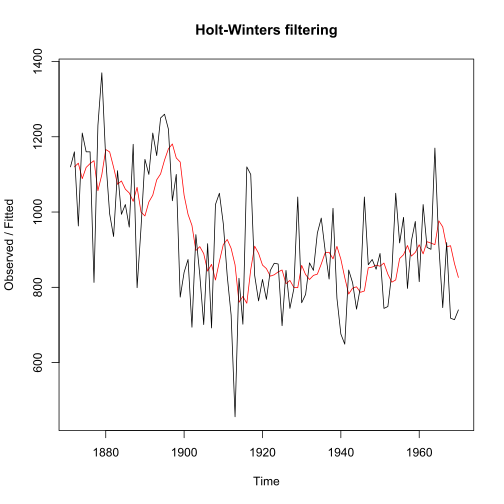
\includegraphics[width=0.7\textwidth]{figures/TimeSeriesNileHoltWinters-1} 

\end{knitrout}
Note that we must explicitly set \Rarg{beta} and \Rarg{gamma} to \Rarg{FALSE} to get the simple exponential smoother. 
 
 
Adding a linear trend is fairly simple, but the seasonal component can be expressed as either an additive or a multiplicative term. The two forms would be 
$$y_t = \mu_t + \beta_t t +S_{t-p} + e_t$$ 
and 
$$y_t = (\mu_t + \beta_t t) S_{t-p} + e_t$$ 
respectively , where the $\mu_t$ is found using a deseasonalised version of the simple exponential smoother 
$$\mu_t = \alpha (y_t - S_{t-p}) + (1-\alpha) (\mu_{t-1} + \beta_{t-1})$$ 
for the additive model and 
$$\mu_t = \alpha \frac{y_t }{ S_{t-p}} + (1-\alpha) (\mu_{t-1} + \beta_{t-1})$$ 
for the multiplicative model. 
 
\begin{knitrout}
\definecolor{shadecolor}{rgb}{0.969, 0.969, 0.969}\color{fgcolor}\begin{kframe}
\begin{alltt}
\hlstd{> }\hlstd{AustRes.hw1} \hlkwb{=} \hlkwd{HoltWinters}\hlstd{(austres)}
\hlstd{> }\hlstd{AustRes.hw1}
\end{alltt}
\begin{verbatim}
Holt-Winters exponential smoothing with trend and additive seasonal component.

Call:
HoltWinters(x = austres)

Smoothing parameters:
 alpha: 0.9672
 beta : 0.2585
 gamma: 1

Coefficients:
         [,1]
a  17662.6967
b     45.7125
s1    -4.3828
s2     0.5476
s3     3.8737
s4    -1.1967
\end{verbatim}
\begin{alltt}
\hlstd{> }\hlkwd{plot}\hlstd{(AustRes.hw1)}
\end{alltt}
\end{kframe}
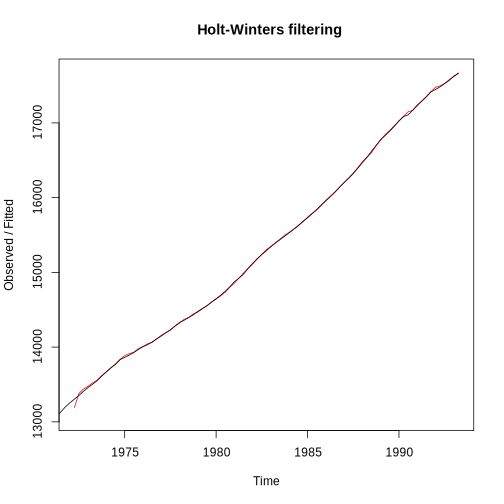
\includegraphics[width=0.7\textwidth]{figures/TimeSeriesAustResHW-1} 
\begin{kframe}\begin{alltt}
\hlstd{> }\hlstd{AustRes.hw2} \hlkwb{=} \hlkwd{HoltWinters}\hlstd{(austres,} \hlkwc{seasonal}\hlstd{=}\hlstr{"mult"}\hlstd{)}
\hlstd{> }\hlstd{AustRes.hw2}
\end{alltt}
\begin{verbatim}
Holt-Winters exponential smoothing with trend and multiplicative seasonal component.

Call:
HoltWinters(x = austres, seasonal = "mult")

Smoothing parameters:
 alpha: 0.9622
 beta : 0.2593
 gamma: 1

Coefficients:
        [,1]
a  1.766e+04
b  4.564e+01
s1 9.997e-01
s2 1.000e+00
s3 1.000e+00
s4 9.999e-01
\end{verbatim}
\begin{alltt}
\hlstd{> }\hlkwd{plot}\hlstd{(AustRes.hw2)}
\end{alltt}
\end{kframe}
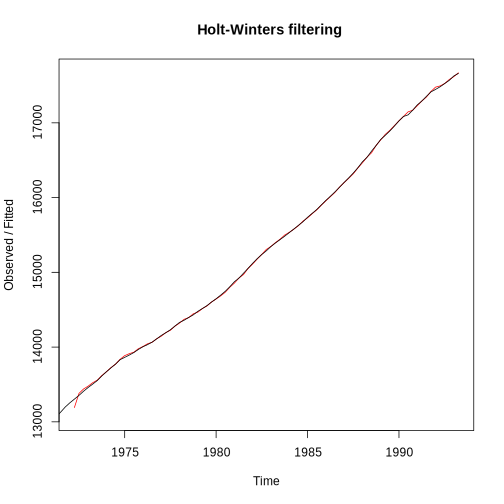
\includegraphics[width=0.7\textwidth]{figures/TimeSeriesAustResHW-2} 

\end{knitrout}
 
 
 
 
 
 
\section{Autoregressive models} 
 
ar() 
 
\section{Basic ARIMA models} 
 
ARIMA models require the autoregressive and moving average components to be built on a stationary series. We often need to create a stationary series using differencing as seen in Section~\ref{Stationarity} above. 
arima() 
 
\section{Seasonality and ARIMA modelling} 
 


